\documentclass{article}
\usepackage{amsmath}
\usepackage{amssymb}
\usepackage{hyperref}
\usepackage{pdfpages}
\usepackage{graphicx}
\usepackage{subcaption}
\usepackage{float}

\title{Assignment 3A}
\author{Botond Lovász}
\date{\today}

\begin{document}

\maketitle

\section{Principal Component Analysis}

\subsection{Question 3.1.1}


It translates the dataset so that its mean is at the origin of the coordinate space. This is important because PCA seeks to find the directions (principal components) that maximize the variance of the data. If the data is not centered, the first principal component might simply point towards the mean of the data rather than capturing the true direction of maximum variance.

This can lead to misleading results and the dimensionality reduction may not effectively capture the underlying patterns, leading to poor performance in subsequent analyses or models.
    
When the data is centered, \(\bar{X} = 0\) and \(\bar{Y} = 0\). This simplifies the (estimated) covariance calculation to:
\[
\text{Cov}(X, Y) = \frac{1}{n-1} \sum_{i=1}^{n} X_i Y_i
\]


\subsection{Question 3.1.2}

SVD decomposes a matrix \( A \) into three matrices: \( U \), \( \Sigma \), and \( V^T \), such that \( A = U \Sigma V^T \). The principal components are derived from the eigenvectors of the covariance matrix. For a data matrix \( A \), the covariance matrix for the rows is \( A^T A \), and for the columns, it is \( A A^T \).

The SVD of the transpose \( A^T \) is \( V \Sigma^T U^T \). This implies that the roles of \( U \) and \( V \) are swapped, and the singular values remain the same (though the matrix \( \Sigma \) is transposed).

The eigenvectors of the covariance matrix \( A^T A \) (for rows) and \( A A^T \) (for columns) are derived from \( V \) and \( U \) respectively.

Thus, a single SVD operation is sufficient to perform PCA on both the rows and columns of a data matrix. 

\subsection{Question 3.1.3}


Given the dataset \( Y = \{y_1, \ldots, y_n\} \) with zero-centered data, the variance is defined as:
\[
\text{Var}(Y) = \sum_{y \in Y} \|y - \bar{y}\|^2_2 = \sum_{y \in Y} \|y\|^2_2
\]
Since the data is zero-centered, \(\bar{y} = 0\).

The variance of \( Y \) can be expressed as the sum of the squared norms of its columns:
\[
\text{Var}(Y) = \sum_{i=1}^{n} \|y_i\|^2_2 = \text{trace}(Y^T Y)
\]
Using the SVD, \( Y^T Y = (U \Sigma V^T)^T (U \Sigma V^T) = V \Sigma^T U^T U \Sigma V^T = V \Sigma^T \Sigma V^T \).
Since \( U \) is orthogonal, \( U^T U = I \).
The trace of a matrix is invariant under cyclic permutations, so:
\[
\text{trace}(Y^T Y) = \text{trace}(\Sigma^T \Sigma) = \sum_{i=1}^{d} \sigma_i^2
\]

So, the variance of the dataset \( Y \) can be expressed as the sum of the squares of the singular values of \( Y \):
\[
\text{Var}(Y) = \sum_{i=1}^{d} \sigma_i^2
\]

\newpage

\subsection{Question 3.1.4}

The first \( k \) principal components are the first \( k \) columns of \( U \). The matrix \( W \) is formed by these \( k \) principal components, i.e., \( W = U_k \), where \( U_k \) is the \( d \times k \) matrix consisting of the first \( k \) columns of \( U \).

The projected data \( X \) is given by \( X = W^T Y = U_k^T Y \). Substituting the SVD of \( Y \), we have:
\[
X = U_k^T (U \Sigma V^T) = U_k^T U \Sigma V^T
\]
Since \( U \) is orthogonal, \( U_k^T U \) results in a \( k \times d \) matrix with the first \( k \) rows of the identity matrix, effectively selecting the first \( k \) rows of \( \Sigma \).

The variance of the projected data \( X \) is the trace of the covariance matrix of \( X \), which is \( X X^T \). Substituting for \( X \), we have:
\[
X X^T = (U_k^T U \Sigma V^T)(V \Sigma^T U^T U_k) = U_k^T U \Sigma \Sigma^T U^T U_k
\]
Since \( U \) is orthogonal, \( U^T U = I \), thus:
\[
X X^T = U_k^T \Sigma \Sigma^T U_k
\]
The matrix \( \Sigma \Sigma^T \) is a diagonal matrix with the squares of the singular values \(\sigma_1^2, \sigma_2^2, \ldots, \sigma_d^2\) on the diagonal. The trace of \( U_k^T \Sigma \Sigma^T U_k \) is the sum of the first \( k \) diagonal elements of \( \Sigma \Sigma^T \), which are \(\sigma_1^2, \sigma_2^2, \ldots, \sigma_k^2\).

The variance of the projected data \( X \) is indeed given by the sum of the squares of the first \( k \) singular values of \( Y \):
\[
\text{Var}(X) = \sum_{i=1}^{k} \sigma_i^2
\]

\subsection{Question 3.1.5}

In matrix form, the residual data is \( Z = Y - W W^T Y \).

The projection matrix \( W W^T \) projects \( Y \) onto the subspace spanned by the first \( k \) principal components. The residuals \( Z \) are the components of \( Y \) orthogonal to this subspace.

The variance of the residual data \( Z \) is the trace of the covariance matrix of \( Z \), which is \( Z Z^T \). Substituting for \( Z \), we have:
\[
Z = Y - W W^T Y = (I - W W^T) Y
\]
Therefore, the covariance matrix of \( Z \) is:
\[
Z Z^T = (I - W W^T) Y Y^T (I - W W^T)^T
\]
Using the SVD of \( Y = U \Sigma V^T \), we have:
\[
Y Y^T = U \Sigma V^T V \Sigma^T U^T = U \Sigma \Sigma^T U^T
\]
The matrix \( \Sigma \Sigma^T \) is diagonal with \(\sigma_1^2, \sigma_2^2, \ldots, \sigma_d^2\) on the diagonal.

The variance of the residual data \( Z \) is the sum of the squares of the singular values corresponding to the dimensions not captured by the first \( k \) principal components:
\[
\text{Var}(Z) = \sum_{i=k+1}^{d} \sigma_i^2
\]

So, the variance of the residual data \( Z \) is indeed given by the sum of the squares of the singular values from \( k+1 \) to \( d \). Therefore, the variance of the original data is the sum of the variance explained by PCA and the variance of the residual data:
\[
\text{Var}(Y) = \text{Var}(X) + \text{Var}(Z)
\]

\section{Classifying non-linearly-separable data with a linear classifier}

\subsection{Question 3.2.6}

To map the data into a two-dimensional space where they become linearly separable, we used a simple transformation by squaring the attributes. We chose this because we see from the given figure, that the data is centered around the same point and it is distributed in 2 different circles. We can easily separate 2 circles by their radius, but the task asked to map it into a 2D space, so we take the square of the attributes to get a 2D space and still be able to separate them based on the original radius. (We could have also used the absolute value of the attributes to get a 2D space, or map it into polar coordinates.)

\begin{itemize}
    \item For each data point \((x, y)\), compute new features by squaring the original attributes:
    \[
    \phi_1(x, y) = x^2, \quad \phi_2(x, y) = y^2
    \]

    \item Each data point \((x, y)\) in the original space is transformed to \((x^2, y^2)\) in the new space.
\end{itemize}

\begin{figure}[H]
    \centering
    \begin{subfigure}{0.45\textwidth}
        \centering
        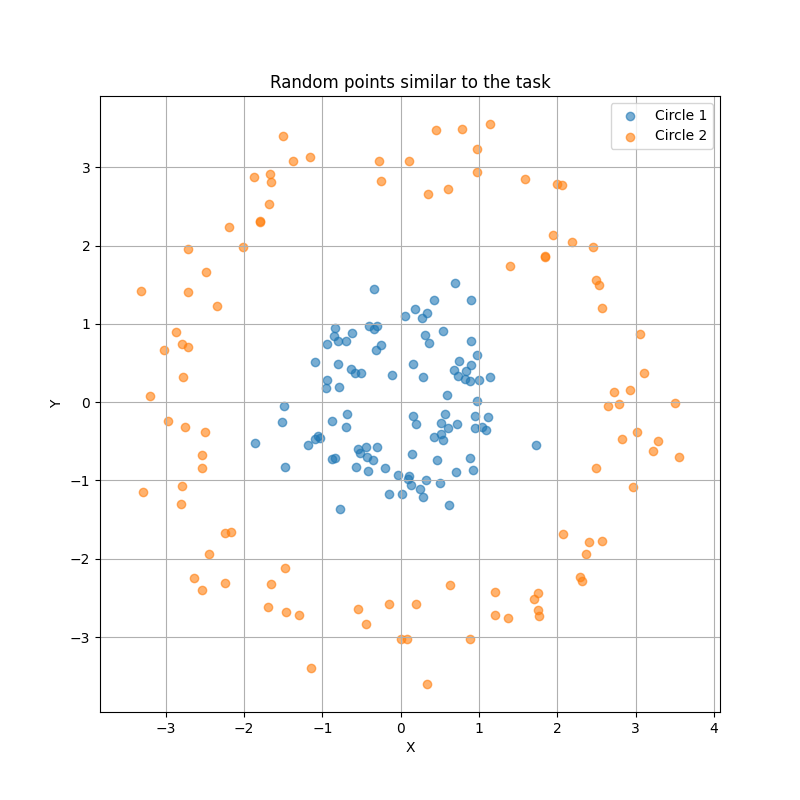
\includegraphics[width=\textwidth]{random_points.png}
        \caption{Points similar to the task}
    \end{subfigure}
    \hfill
    \begin{subfigure}{0.45\textwidth}
        \centering
        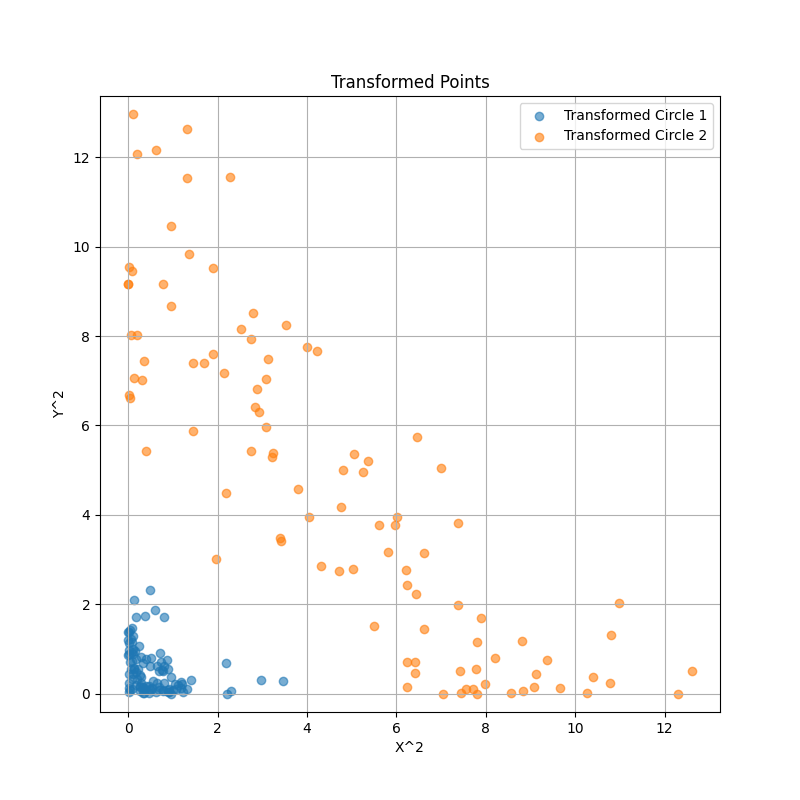
\includegraphics[width=\textwidth]{transformed_points.png}
        \caption{Transformed points}
    \end{subfigure}
    \caption{Figures showing the points and their transformed counterparts}
\end{figure}

\subsection{Question 3.2.7}

\begin{figure}[H]
    \centering
    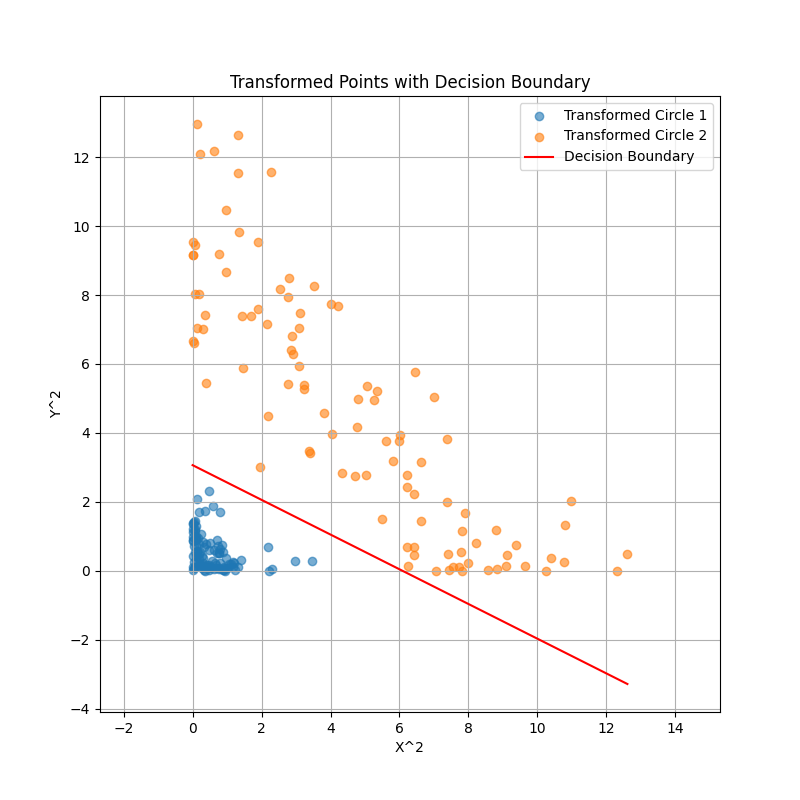
\includegraphics[width=0.8\textwidth]{transformed_points_with_decision_boundary.png}
    \caption{Transformed points with decision boundary}
\end{figure}

\begin{itemize}
    \item Given a new data point \((x, y)\) in the original space, apply the same transformation used during training:
    \[
    \phi_1(x, y) = x^2, \quad \phi_2(x, y) = y^2
    \]
    This maps the point to the transformed space where the data is linearly separable.

    \item Use the trained linear classifier to predict the label of the transformed data point \((\phi_1, \phi_2)\).
    The classifier uses a decision boundary, typically defined by a weight vector \( \mathbf{w} \) and a bias \( b \). The decision function is:
    \[
    f(\phi_1, \phi_2) = \mathbf{w} \cdot \begin{bmatrix} \phi_1 \\ \phi_2 \end{bmatrix} + b
    \]
    If \( f(\phi_1, \phi_2) > 0 \), classify the point as one class; otherwise, classify it as the other class.

    \item In our case, the decision boundary is a line, and the points are classified based on which side of the line they lie on. We can easily compute this by using the equation of the line and calculating the \(y'\) value for the input \(x^2\) and seeing if it is greater than the transformed \(y^2\) value.
\end{itemize}

\begin{figure}[H]
    \centering
    \begin{subfigure}{0.45\textwidth}
        \centering
        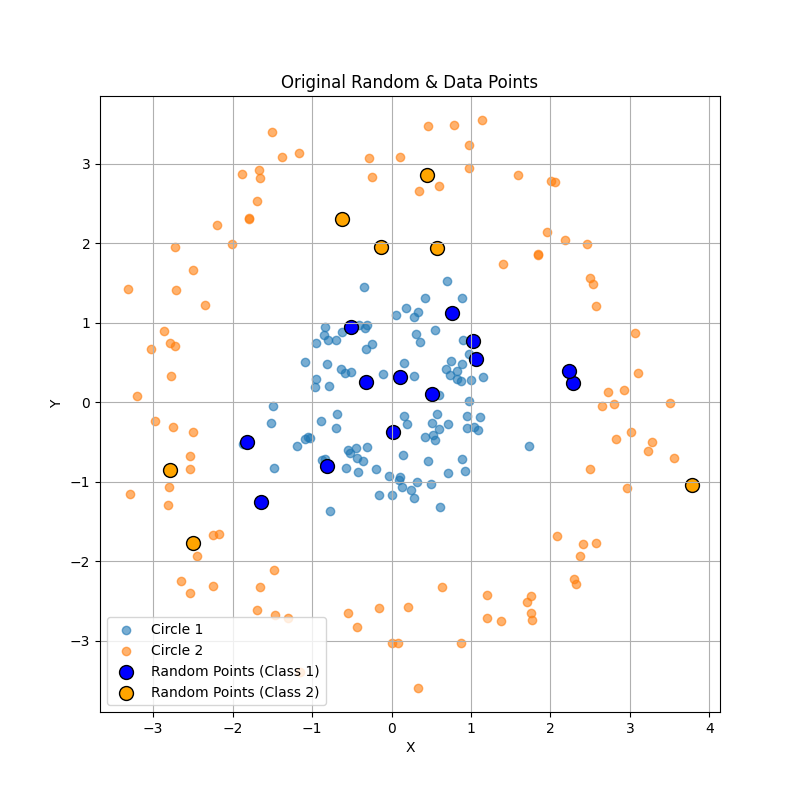
\includegraphics[width=\textwidth]{original_random_data_points.png}
        \caption{Random points}
    \end{subfigure}
    \hfill
    \begin{subfigure}{0.45\textwidth}
        \centering
        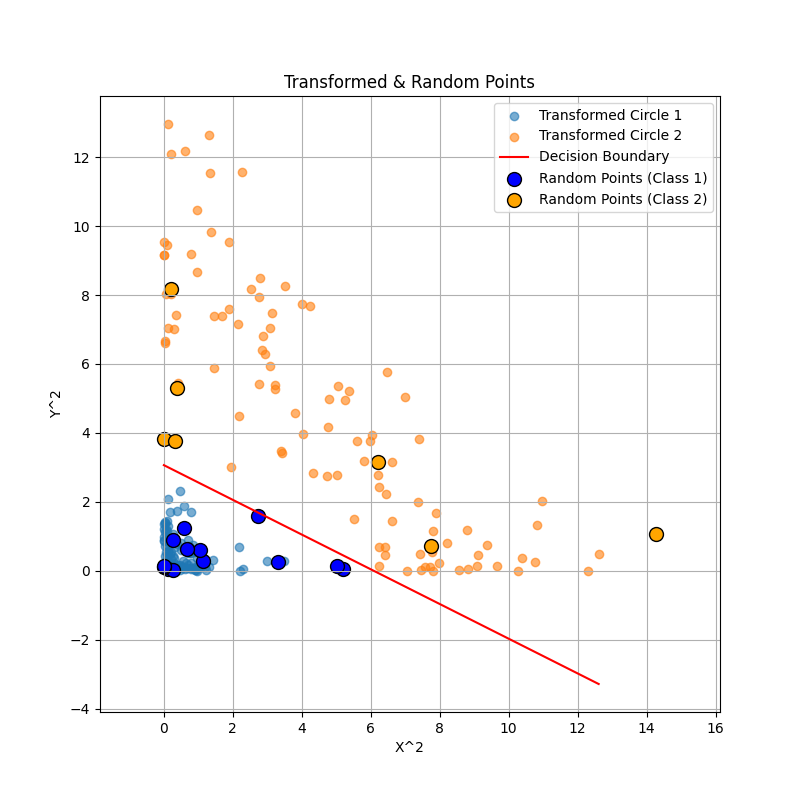
\includegraphics[width=\textwidth]{transformed_random_data_points.png}
        \caption{Transformed Random points}
    \end{subfigure}
    \caption{Figures showing the random points and their transformed counterparts with classification}
\end{figure}

\newpage

\section{Spectral graph analysis}

\subsection{Question 3.3.8}

The normalized Laplacian \( L \) is defined as:

\[
L = I - \frac{1}{d} A
\]

where \( I \) is the identity matrix.

\[
x^T L x = x^T \left(I - \frac{1}{d} A\right) x = x^T I x - \frac{1}{d} x^T A x
\]

Since \(A\) is the adjacency matrix is symmetric (of an undirected graph) and \(a_{ij} = 1\) if \((i, j) \in E\) or \((j, i) \in E\) and \(0\) otherwise.

\[
x^T A x = \sum_{i=1}^{|V|} \sum_{j=1}^{|V|} a_{ij} x_i x_j = 2 \sum_{(u,v) \in E} x_u x_v
\]

\[
x^T I x = \sum_{v=1}^{|V|} x_v^2
\]

\[
x^T L x = \sum_{v=1}^{|V|} x_v^2 - \frac{2}{d} \sum_{(u,v) \in E} x_u x_v
\]

Summing over all edges \((u, v) \in E\):
\[
\sum_{(u,v) \in E} (x_u - x_v)^2 = \sum_{(u,v) \in E} (x_u^2 + x_v^2 - 2x_u x_v)
\]

Since \( G \) is \( d \)-regular, each vertex \( i \) appears in exactly \( d \) edges:
\[
\sum_{(u,v) \in E} x_u^2 + \sum_{(u,v) \in E} x_v^2 = d \sum_{v=1}^{|V|} x_v^2
\]

Therefore:
\[
\sum_{(u,v) \in E} (x_u - x_v)^2 = d \sum_{v=1}^{|V|} x_v^2 - 2 \sum_{(u,v) \in E} x_u x_v
\]

Divide by \( d \) to match the form:
\[
\frac{1}{d} \sum_{(u,v) \in E} (x_u - x_v)^2 = \sum_{v=1}^{|V|} x_v^2 - \frac{2}{d} \sum_{(u,v) \in E} x_u x_v
\]

This matches the expression for \( x^T L x \), proving the statement.

\subsection{Question 3.3.9}

A symmetric matrix \( L \) is positive semidefinite if for all vectors \( x \in \mathbb{R}^{|V|} \), the quadratic form \( x^T L x \geq 0 \).

The normalized Laplacian \( L = I - \frac{1}{d} A \) is symmetric because both \( I \) (the identity matrix) and \( A \) (the adjacency matrix of an undirected graph) are symmetric matrices.

From the previous derivation, we have shown that for any vector \( x \in \mathbb{R}^{|V|} \):

\[
x^T L x = \frac{1}{d} \sum_{(u,v) \in E} (x_u - x_v)^2
\]

The expression \((x_u - x_v)^2\) is always non-negative for any real numbers \(x_u\) and \(x_v\). Therefore, the sum \(\sum_{(u,v) \in E} (x_u - x_v)^2\) is non-negative. \(d\) is a positive constant as it is the degree of the graph.

Since \( x^T L x = \frac{1}{d} \sum_{(u,v) \in E} (x_u - x_v)^2 \geq 0 \) for all vectors \( x \), it follows that the normalized Laplacian \( L \) is positive semidefinite.

\subsection{Question 3.3.10}

A \textbf{non-trivial vector} \( x_* \) in the context of minimizing \( x^T L x \) refers to a vector that is not the trivial solution, which is typically the zero vector or any constant vector. A vector \( x_* \) is non-trivial if it is not a constant vector.

The vector \( x_* \) can be used to embed the vertices of the graph into the real line. This embedding assigns a real number to each vertex, effectively placing the vertices along a line.

The value \( x_{*i} \) represents the position of vertex \( i \) on the real line. This embedding can be meaningful if it reflects the graph's structure, with closely connected vertices having similar values.

Equation (2) states:
\[
x^T L x = \frac{1}{d} \sum_{(u,v) \in E} (x_u - x_v)^2
\]

The expression \( \sum_{(u,v) \in E} (x_u - x_v)^2 \) measures the total squared difference between connected vertices. Minimizing \( x^T L x \) minimizes these differences, leading to an embedding where connected vertices are placed close together on the real line.

By minimizing \( x^T L x \), the embedding \( x_* \) captures the graph's connectivity structure. Vertices that are directly connected or part of the same cluster will have similar values, reflecting their proximity in the graph.

This embedding is useful for visualizing the graph's structure and identifying clusters or communities within the graph.


\appendix
\section{Jupyter Notebook Output}

\includepdf[pages=-]{test.pdf}

\end{document}